% Document/LinearAlgebra/VectorSpaces/QuotientSpaces/IsomorphismTheorems.tex
% Phase 12: All Four Isomorphism Theorems

\newpage
\section{Isomorphism Theorems}

\begin{remark}[Overview]
    The four isomorphism theorems are the structural backbone of the subject. They describe
    how quotient spaces interact with subspaces, sums, intersections, and nested inclusions.
    Each theorem identifies a natural isomorphism between two quotient spaces that might
    appear unrelated at first glance.

    \begin{itemize}
        \item The \textbf{First Isomorphism Theorem} ($\QuotientSpace{U}{\Ker{T}} \cong \Rng{T}$)
              says that every linear map factors as a surjection followed by an injection, with
              the quotient by the kernel as the intermediate space. This is the most frequently
              used of the four theorems.
        \item The \textbf{Second Isomorphism Theorem}
              ($\QuotientSpace{(U+W)}{W} \cong \QuotientSpace{U}{(U \Intersect W)}$)
              compares two ways of ``modding out'' by $W$: starting from $U + W$ or starting
              from $U$. As a corollary, it yields the Grassmann dimension formula.
        \item The \textbf{Third Isomorphism Theorem}
              ($\QuotientSpace{(\QuotientSpace{V}{U})}{(\QuotientSpace{W}{U})} \cong \QuotientSpace{V}{W}$)
              says that taking quotients in two stages is the same as taking the quotient in
              one step --- ``quotienting by a quotient.''
        \item The \textbf{Fourth Isomorphism Theorem} (Lattice Correspondence) establishes
              a bijection between the subspaces of $\QuotientSpace{V}{W}$ and the subspaces
              of $V$ that contain $W$. This is a lattice isomorphism: it preserves sums,
              intersections, and inclusions.
    \end{itemize}

    All proofs follow the same strategy: define a linear map, identify its kernel and image,
    and invoke the universal property of quotient spaces
    (Theorem~\ref{thm:quotient-universal}).
\end{remark}

\subsection{First Isomorphism Theorem}

\begin{center}
\begin{tikzcd}
U \arrow[r, "T"] \arrow[d, "\pi"'] & V \\
\QuotientSpace{U}{\Ker{T}} \arrow[ru, "\cong"', "\tilde{T}"]
\end{tikzcd}
\end{center}

\begin{theorem}[First Isomorphism Theorem]\label{thm:first-iso}
    For any linear map $T: U \to V$:
    \[
        \QuotientSpace{U}{\Ker{T}} \cong \Rng{T}
    \]
\end{theorem}

\begin{proof}
    Apply the Universal Property (Theorem~\ref{thm:quotient-universal}) with $W = \Ker{T}$ and $X = V$.
    
    Since $\Ker{T} \subseteq \Ker{T}$, there exists a unique linear map 
    $\tilde{T}: \QuotientSpace{U}{\Ker{T}} \to V$ such that $T = \Composition{\tilde{T}}{\pi}$.
    
    By part (4) of the universal property: $\tilde{T}$ is injective since $\Ker{T} = \Ker{T}$.
    
    The image of $\tilde{T}$ equals the image of $T$:
    \[
        \Rng{\tilde{T}} = \Set{\tilde{T}(\EquivClass{u}) \mid u \in U} = \Set{T(u) \mid u \in U} = \Rng{T}
    \]
    
    Thus $\tilde{T}: \QuotientSpace{U}{\Ker{T}} \to \Rng{T}$ is a bijective linear map,
    hence an isomorphism.
\end{proof}

\begin{corollary}[Rank-Nullity via First Isomorphism Theorem]\label{cor:rank-nullity-iso}
    For any linear map $T: U \to V$:
    \[
        \Dim[K]{\Ker{T}} + \Dim[K]{\Rng{T}} = \Dim[K]{U}
    \]
    That is: $\Nullity{T} + \Rank{T} = \Dim[K]{U}$.
\end{corollary}

\begin{proof}
    By the First Isomorphism Theorem: $\QuotientSpace{U}{\Ker{T}} \cong \Rng{T}$.
    
    Thus $\Dim[K]{\QuotientSpace{U}{\Ker{T}}} = \Dim[K]{\Rng{T}}$.
    
    By the Quotient Dimension Formula (Theorem~\ref{thm:quotient-dim}):
    \[
        \Dim[K]{\Ker{T}} + \Dim[K]{\QuotientSpace{U}{\Ker{T}}} = \Dim[K]{U}
    \]
    
    Substituting: $\Dim[K]{\Ker{T}} + \Dim[K]{\Rng{T}} = \Dim[K]{U}$.
\end{proof}

\begin{remark}[Two Proofs of Rank-Nullity]
    We now have two proofs of the Rank-Nullity Theorem:
    \begin{enumerate}
        \item \textbf{Direct proof} (Theorem~\ref{thm:rank-nullity}): Extend a basis of $\Ker{T}$
              and show the images of the extension vectors form a basis of $\Rng{T}$.
        \item \textbf{Via isomorphism theorem} (Corollary~\ref{cor:rank-nullity-iso}): Use
              $\QuotientSpace{U}{\Ker{T}} \cong \Rng{T}$ and the quotient dimension formula.
    \end{enumerate}
    Both approaches are valuable and highlight different aspects of the structure.
\end{remark}

\begin{example}[First Isomorphism Theorem in $\bb{R}^3$]\label{ex:first-iso}
    Define $T: \bb{R}^3 \to \bb{R}^2$ by $T(x, y, z) = (x + y,\; y + z)$.

    \textbf{Kernel:} $T(x,y,z) = (0,0)$ iff $x = -y$ and $z = -y$, so
    $\Ker{T} = \Span[\bb{R}]{\Set{(1, -1, 1)}}$, a line through the origin.

    \textbf{Range:} $T$ is surjective since $T(1,0,0) = (1,0)$ and $T(0,0,1) = (0,1)$,
    so $\Rng{T} = \bb{R}^2$.

    \textbf{The isomorphism explicitly:}
    Each coset in $\QuotientSpace{\bb{R}^3}{\Ker{T}}$ is a line parallel to $(1,-1,1)$.
    The induced map $\tilde{T}: \QuotientSpace{\bb{R}^3}{\Ker{T}} \to \bb{R}^2$ sends
    \[
        \Coset{(x,y,z)}{\Ker{T}} \;\longmapsto\; (x+y,\; y+z)
    \]
    For instance, $\Coset{(1,0,0)}{\Ker{T}} = \Set{(1+t,\; -t,\; t) \mid t \in \bb{R}}$
    maps to $(1,0)$, and every point on that line maps to $(1,0)$.

    Dimension check: $\Dim[\bb{R}]{\QuotientSpace{\bb{R}^3}{\Ker{T}}} = 3 - 1 = 2 = \Dim[\bb{R}]{\bb{R}^2}$.

    % Projection convention:
    %   x-axis -> (1, 0) in TikZ     (horizontal right)
    %   y-axis -> (0.7, 0.5) in TikZ (diagonal up-right)
    %   z-axis -> (0, 1) in TikZ     (vertical up)
    %
    % Projected points:
    %   (0,0,0) -> (0, 0)
    %   (1,0,0) -> (1, 0)
    %   (0,1,0) -> (0.7, 0.5)
    %   (1,-1,1) -> (1 - 0.7 + 0, 0 - 0.5 + 1) = (0.3, 0.5)
    %
    % Direction of ker T = span{(1,-1,1)} projected: (0.3, 0.5)
    % Scaled by 4 for line length: endpoints at ±(1.2, 2.0) from base point

    \begin{center}
    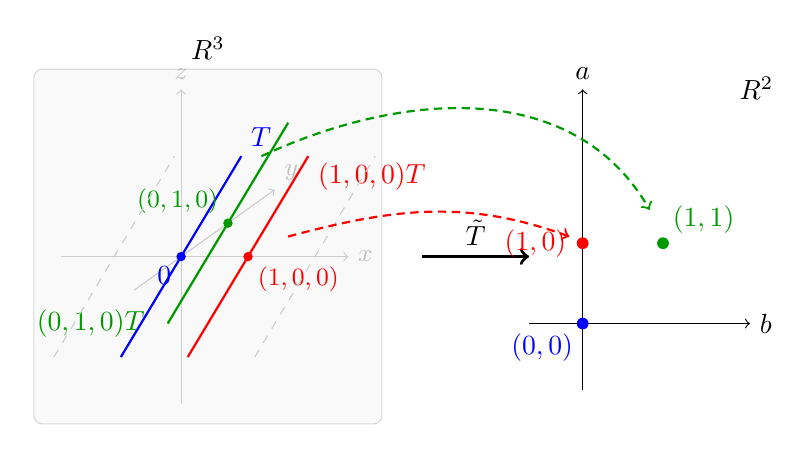
\begin{tikzpicture}[scale=0.85]

        % Bounding region
        \draw[gray!30, fill=gray!5, rounded corners=3pt] (-2.2,-2.5) rectangle (3,2.8);
        \node[above] at (0.4,2.8) {$\bb{R}^3$};

        % Faded coordinate axes
        \draw[->, gray!40] (-1.8,0) -- (2.5,0) node[right, gray!50] {\small $x$};
        \draw[->, gray!40] (0,-2.2) -- (0,2.5) node[above, gray!50] {\small $z$};
        \draw[->, gray!40] (-0.7,-0.5) -- (1.4,1.0) node[above right, gray!50] {\small $y$};

        % Coset lines: all parallel with direction (0.3, 0.5) scaled
        % Using direction (0.9, 1.5) for visible length

        % Blue: ker T through origin (0,0)
        \draw[blue, thick] (-0.9,-1.5) -- (0.9,1.5);
        \node[blue, above right] at (0.9,1.5) {$\Ker{T}$};
        \fill[blue] (0,0) circle (2pt) node[below left] {$0$};

        % Red: coset through (1,0,0) projected to (1, 0)
        \draw[red, thick] (0.1,-1.5) -- (1.9,1.5);
        \node[red, right] at (1.9,1.2) {$\Coset{(1,0,0)}{\Ker{T}}$};
        \fill[red] (1,0) circle (2pt) node[below right] {\small $(1,0,0)$};

        % Green: coset through (0,1,0) projected to (0.7, 0.5)
        \draw[green!60!black, thick] (-0.2,-1.0) -- (1.6,2.0);
        \node[green!60!black, left] at (-0.4,-1.0) {$\Coset{(0,1,0)}{\Ker{T}}$};
        \fill[green!60!black] (0.7,0.5) circle (2pt) node[above left] {\small $(0,1,0)$};

        % Dashed cosets for texture
        \draw[gray!40, dashed] (-1.9,-1.5) -- (-0.1,1.5);
        \draw[gray!40, dashed] (1.1,-1.5) -- (2.9,1.5);

        % Arrow
        \draw[->, very thick] (3.6,0) -- (5.2,0) node[midway, above] {$\tilde{T}$};

        % Right side: R^2
        \draw[->] (6,-2) -- (6,2.5) node[above] {$a$};
        \draw[->] (5.2,-1) -- (8.5,-1) node[right] {$b$};
        \node[above right] at (8.2,2.2) {$\bb{R}^2$};

        % Target points
        \fill[blue] (6,-1) circle (2.5pt);
        \node[blue, below left] at (6,-1) {$(0,0)$};

        \fill[red] (6,0.2) circle (2.5pt);
        \node[red, left] at (5.9,0.2) {$(1,0)$};

        \fill[green!60!black] (7.2,0.2) circle (2.5pt);
        \node[green!60!black, above right] at (7.2,0.2) {$(1,1)$};

        % Colored arrows showing the map
        \draw[->, red, densely dashed, thick] (1.6,0.3) to[out=15, in=160] (5.8,0.3);
        \draw[->, green!60!black, densely dashed, thick] (1.2,1.5) to[out=25, in=120] (7.0,0.7);
    \end{tikzpicture}
    \end{center}
\end{example}

\subsection{Second Isomorphism Theorem}

\begin{center}
\begin{tikzcd}
& U + W \arrow[d, "\pi_W"] \\
U \arrow[ru, hook] \arrow[r, "\iota"] & \QuotientSpace{(U+W)}{W} \\
U \Intersect W \arrow[u, hook] \arrow[r, "\pi_{U \Intersect W}"'] & \QuotientSpace{U}{(U \Intersect W)} \arrow[u, "\cong"']
\end{tikzcd}
\end{center}

\begin{theorem}[Second Isomorphism Theorem]\label{thm:second-iso}
    Let $U, W \Subspace[K] V$. Then:
    \[
        \QuotientSpace{(U + W)}{W} \cong \QuotientSpace{U}{(U \Intersect W)}
    \]
\end{theorem}

\begin{proof}
    Consider the composition:
    \[
        T: U \xhookrightarrow{\iota} U + W \xrightarrow{\pi_W} \QuotientSpace{(U+W)}{W}
    \]
    where $\iota$ is the inclusion and $\pi_W$ is the canonical projection.
    
    \textbf{$T$ is surjective:}
    For any $\EquivClass{u + w} \in \QuotientSpace{(U+W)}{W}$ with $u \in U$ and $w \in W$:
    \[
        \EquivClass{u + w} = \EquivClass{u} + \EquivClass{w} = \EquivClass{u} + \EquivClass{0} = \EquivClass{u} = T(u)
    \]
    since $w \in W$ implies $\EquivClass{w} = \EquivClass{0}$.
    
    \textbf{$\Ker{T} = U \Intersect W$:}
    \begin{align*}
        u \in \Ker{T} &\Leftrightarrow \pi_W(\iota(u)) = \EquivClass{0} \\
                      &\Leftrightarrow \EquivClass{u} = \EquivClass{0} \text{ in } \QuotientSpace{(U+W)}{W} \\
                      &\Leftrightarrow u \in W \\
                      &\Leftrightarrow u \in U \Intersect W
    \end{align*}
    
    By the First Isomorphism Theorem:
    \[
        \QuotientSpace{U}{\Ker{T}} = \QuotientSpace{U}{(U \Intersect W)} \cong \Rng{T} = \QuotientSpace{(U+W)}{W}
    \]
\end{proof}

\begin{example}[Second Isomorphism Theorem in $\bb{R}^3$]\label{ex:second-iso}
    Let $V = \bb{R}^3$, $U = \Set{(x,y,0) \mid x,y \in \bb{R}}$ (the $xy$-plane),
    and $W = \Set{(x,0,z) \mid x,z \in \bb{R}}$ (the $xz$-plane).

    Then $U + W = \bb{R}^3$ and $U \Intersect W = \Set{(x,0,0) \mid x \in \bb{R}}$ (the $x$-axis).

    The theorem says $\QuotientSpace{(U+W)}{W} \cong \QuotientSpace{U}{(U \Intersect W)}$, i.e.,
    $\QuotientSpace{\bb{R}^3}{W} \cong \QuotientSpace{U}{(U \Intersect W)}$.

    \textbf{Left side:} $\QuotientSpace{\bb{R}^3}{W}$ collapses the $xz$-plane to zero.
    Each coset $\Coset{(a,b,c)}{W} = \Set{(a+s, b, c+t) \mid s,t \in \bb{R}}$ is determined
    by $b$ alone, so $\QuotientSpace{\bb{R}^3}{W} \cong \bb{R}$ (the $y$-direction).

    \textbf{Right side:} $\QuotientSpace{U}{(U \Intersect W)}$ collapses the $x$-axis within
    the $xy$-plane. Each coset $\Coset{(a,b,0)}{U \Intersect W} = \Set{(a+s, b, 0) \mid s \in \bb{R}}$
    is determined by $b$ alone, so $\QuotientSpace{U}{(U \Intersect W)} \cong \bb{R}$ (again the $y$-direction).

    Both quotients collapse to the same copy of $\bb{R}$---two different ways of ``projecting
    onto the $y$-axis.''

    \begin{center}
    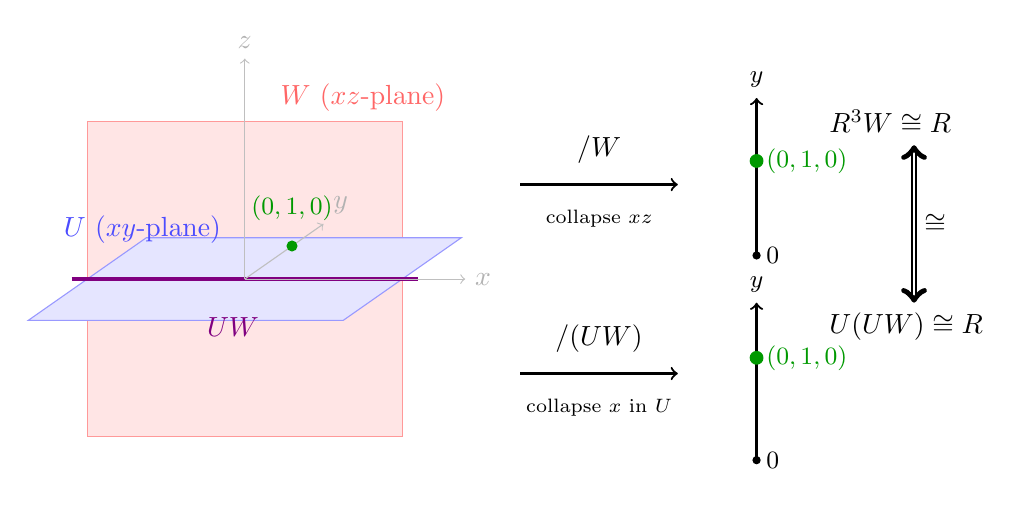
\begin{tikzpicture}[scale=1.0,
        x={(1cm,0cm)},
        y={(0.5cm,0.35cm)},
        z={(0cm,1cm)}]

        % --- Left: R^3 in oblique projection ---

        % xz-plane (W) — a parallelogram in the xz-plane
        \fill[red!10] (-2,0,-2) -- (2,0,-2) -- (2,0,2) -- (-2,0,2) -- cycle;
        \draw[red!40] (-2,0,-2) -- (2,0,-2) -- (2,0,2) -- (-2,0,2) -- cycle;
        \node[red!60] at (1.5,0,2.3) {$W$ ($xz$-plane)};

        % xy-plane (U) — a parallelogram in the xy-plane
        \fill[blue!10] (-2,-1.5,0) -- (2,-1.5,0) -- (2,1.5,0) -- (-2,1.5,0) -- cycle;
        \draw[blue!40] (-2,-1.5,0) -- (2,-1.5,0) -- (2,1.5,0) -- (-2,1.5,0) -- cycle;
        \node[blue!70] at (-2.2,1.8,0) {$U$ ($xy$-plane)};

        % x-axis (intersection) highlighted
        \draw[violet, very thick] (-2.2,0,0) -- (2.2,0,0);
        \node[violet] at (0,-0.3,-0.5) {$U \Intersect W$};

        % Axes
        \draw[->, gray!50] (0,0,0) -- (2.8,0,0) node[right, gray!60] {$x$};
        \draw[->, gray!50] (0,0,0) -- (0,2,0) node[above right, gray!60] {$y$};
        \draw[->, gray!50] (0,0,0) -- (0,0,2.8) node[above, gray!60] {$z$};

        % Sample point
        \fill[green!60!black] (0,1.2,0) circle (2pt);
        \node[green!60!black, above] at (0,1.2,0.2) {\small $(0,1,0)$};

        % --- Arrows to quotients ---
        \draw[->, thick] (3.5,0,1.2) -- (5.5,0,1.2);
        \node[above] at (4.5,0,1.35) {$/W$};
        \node[below, font=\scriptsize] at (4.5,0,1.0) {collapse $xz$};

        \draw[->, thick] (3.5,0,-1.2) -- (5.5,0,-1.2);
        \node[above] at (4.5,0,-1.05) {$/(U \Intersect W)$};
        \node[below, font=\scriptsize] at (4.5,0,-1.4) {collapse $x$ in $U$};

        % --- Top right: R^3 / W ---
        \draw[->, thick] (6.5,0,0.3) -- (6.5,0,2.3) node[above] {\small $y$};
        \fill[green!60!black] (6.5,0,1.5) circle (2.5pt) node[right] {\small $\EquivClass{(0,1,0)}$};
        \fill (6.5,0,0.3) circle (1.5pt) node[right] {\small $\EquivClass{0}$};
        \node[right] at (7.3,0,2) {$\QuotientSpace{\bb{R}^3}{W} \cong \bb{R}$};

        % --- Bottom right: U / (U cap W) ---
        \draw[->, thick] (6.5,0,-2.3) -- (6.5,0,-0.3) node[above] {\small $y$};
        \fill[green!60!black] (6.5,0,-1.0) circle (2.5pt) node[right] {\small $\EquivClass{(0,1,0)}$};
        \fill (6.5,0,-2.3) circle (1.5pt) node[right] {\small $\EquivClass{0}$};
        \node[right] at (7.3,0,-0.6) {$\QuotientSpace{U}{(U \Intersect W)} \cong \bb{R}$};

        % Isomorphism between the two quotients (vertical, between top and bottom)
        \draw[<->, double, thick] (8.5,0,1.7) -- (8.5,0,-0.3)
            node[midway, right] {$\cong$};
    \end{tikzpicture}
    \end{center}

    \begin{center}
    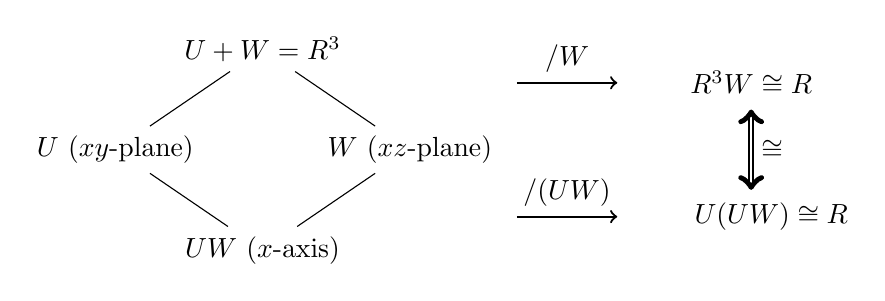
\begin{tikzpicture}[scale=0.85]
        % Diamond diagram
        \node (UW) at (0,3) {$U + W = \bb{R}^3$};
        \node (U)  at (-2.2,1.5) {$U$ ($xy$-plane)};
        \node (W)  at (2.2,1.5) {$W$ ($xz$-plane)};
        \node (UcapW) at (0,0) {$U \Intersect W$ ($x$-axis)};

        \draw (UW) -- (U);
        \draw (UW) -- (W);
        \draw (U) -- (UcapW);
        \draw (W) -- (UcapW);

        % Right: the two quotients
        \draw[->, thick] (3.8,2.5) -- (5.3,2.5) node[midway, above] {$/W$};
        \draw[->, thick] (3.8,0.5) -- (5.3,0.5) node[midway, above] {$/(U \Intersect W)$};

        \node at (7.3,2.5) {$\QuotientSpace{\bb{R}^3}{W} \cong \bb{R}$};
        \node at (7.6,0.5) {$\QuotientSpace{U}{(U \Intersect W)} \cong \bb{R}$};

        % Isomorphism
        \draw[<->, double, thick] (7.3,2.1) -- (7.3,0.9) node[midway, right] {$\cong$};
    \end{tikzpicture}
    \end{center}
\end{example}

\begin{corollary}[Grassmann Formula via Second Isomorphism Theorem]\label{cor:grassmann-iso}
    Let $U, W \Subspace[K] V$. Then:
    \[
        \Dim[K]{U + W} + \Dim[K]{U \Intersect W} = \Dim[K]{U} + \Dim[K]{W}
    \]
    In finite dimensions, this rearranges to
    $\Dim[K]{U + W} = \Dim[K]{U} + \Dim[K]{W} - \Dim[K]{U \Intersect W}$.
\end{corollary}

\begin{proof}
    By the Second Isomorphism Theorem,
    $\QuotientSpace{(U + W)}{W} \cong \QuotientSpace{U}{(U \Intersect W)}$, so the two
    quotients have a common dimension
    \[
        \delta \defeq \Dim[K]{\QuotientSpace{(U + W)}{W}}
        = \Dim[K]{\QuotientSpace{U}{(U \Intersect W)}}
    \]
    By the Quotient Dimension Formula (applied twice):
    \begin{align*}
        \Dim[K]{U + W} &= \Dim[K]{W} + \delta \\
        \Dim[K]{U} &= \Dim[K]{U \Intersect W} + \delta
    \end{align*}
    Substituting both into the desired left-hand side:
    \[
        \Dim[K]{U + W} + \Dim[K]{U \Intersect W}
        = \Dim[K]{W} + \delta + \Dim[K]{U \Intersect W}
        = \Dim[K]{W} + \Dim[K]{U} \qedhere
    \]
\end{proof}

\subsection{Third Isomorphism Theorem}

\begin{remark}[Motivation]
    Suppose we have nested subspaces $U \subseteq W \subseteq V$ and want to form the
    quotient $\QuotientSpace{V}{W}$. We can do this in one step, or in two: first
    collapse $U$ (getting $\QuotientSpace{V}{U}$), then collapse the image of $W$
    (getting $\QuotientSpace{(\QuotientSpace{V}{U})}{(\QuotientSpace{W}{U})}$). The
    third isomorphism theorem says these two procedures give the same result. Intuitively,
    it does not matter whether we collapse a large subspace all at once or in stages ---
    the final quotient depends only on what was collapsed in total.
\end{remark}

\begin{center}
\begin{tikzcd}
V \arrow[r, "\pi_U"] \arrow[d, "\pi_W"'] & \QuotientSpace{V}{U} \arrow[d, "\bar{\pi}"] \\
\QuotientSpace{V}{W} & \QuotientSpace{\QuotientSpace p{V}{U}}{\QuotientSpace p{W}{U}} \arrow[l, "\cong"']
\end{tikzcd}
\end{center}

\begin{theorem}[Third Isomorphism Theorem]\label{thm:third-iso}
    Let $U \subseteq W \subseteq V$ be subspaces. Then:
    \[
        \QuotientSpace{\QuotientSpace p{V}{U}}{\QuotientSpace p{W}{U}} \cong \QuotientSpace{V}{W}
    \]
    where $\QuotientSpace{W}{U} \Subspace[K] \QuotientSpace{V}{U}$ is identified with its image 
    under the natural inclusion.
\end{theorem}

\begin{proof}
    Note that $\QuotientSpace{W}{U} = \Set{\Coset{w}{U} \mid w \in W}$ is naturally a subspace of $\QuotientSpace{V}{U}$.
    
    Consider the canonical projection $\pi_W: V \to \QuotientSpace{V}{W}$.
    
    We apply the Universal Property to factor $\pi_W$ through $\QuotientSpace{V}{U}$.
    
    Since $U \subseteq W = \Ker{\pi_W}$, there exists a unique linear map 
    $\bar{\pi}: \QuotientSpace{V}{U} \to \QuotientSpace{V}{W}$ with $\pi_W = \Composition{\bar{\pi}}{\pi_U}$.
    
    Explicitly: $\bar{\pi}(\Coset{v}{U}) = \Coset{v}{W}$ for all $v \in V$.
    
    \textbf{$\bar{\pi}$ is surjective:}
    For any $\Coset{v}{W} \in \QuotientSpace{V}{W}$: $\bar{\pi}(\Coset{v}{U}) = \Coset{v}{W}$.
    
    \textbf{$\Ker{\bar{\pi}} = \QuotientSpace{W}{U}$:}
    \begin{align*}
        \Coset{v}{U} \in \Ker{\bar{\pi}} &\Leftrightarrow \bar{\pi}(\Coset{v}{U}) = \Coset{0}{W} \\
                                          &\Leftrightarrow \Coset{v}{W} = \Coset{0}{W} \\
                                          &\Leftrightarrow v \in W \\
                                          &\Leftrightarrow \Coset{v}{U} \in \QuotientSpace{W}{U}
    \end{align*}
    
    By the First Isomorphism Theorem applied to $\bar{\pi}$:
    \[
        \QuotientSpace{\QuotientSpace p{V}{U}}{\Ker{\bar{\pi}}} = \QuotientSpace{\QuotientSpace p{V}{U}}{\QuotientSpace p{W}{U}} \cong \Rng{\bar{\pi}} = \QuotientSpace{V}{W}
    \]
\end{proof}

\begin{corollary}[Dimension Cancellation]\label{cor:dim-cancel}
    Let $U \subseteq W \subseteq V$ be subspaces. Then:
    \[
        \Dim[K]{\QuotientSpace{V}{U}} = \Dim[K]{\QuotientSpace{V}{W}} + \Dim[K]{\QuotientSpace{W}{U}}
    \]
\end{corollary}

\begin{proof}
    By the Third Isomorphism Theorem: 
    $\QuotientSpace{\QuotientSpace p{V}{U}}{\QuotientSpace p{W}{U}} \cong \QuotientSpace{V}{W}$.
    
    By the Quotient Dimension Formula:
    \[
        \Dim[K]{\QuotientSpace{W}{U}} + \Dim[K]{\QuotientSpace{\QuotientSpace p{V}{U}}{\QuotientSpace p{W}{U}}} = \Dim[K]{\QuotientSpace{V}{U}}
    \]
    
    Since $\Dim[K]{\QuotientSpace{\QuotientSpace p{V}{U}}{\QuotientSpace p{W}{U}}} = \Dim[K]{\QuotientSpace{V}{W}}$:
    \[
        \Dim[K]{\QuotientSpace{W}{U}} + \Dim[K]{\QuotientSpace{V}{W}} = \Dim[K]{\QuotientSpace{V}{U}}
    \]
\end{proof}

\begin{example}[Third Isomorphism Theorem in $\bb{R}^3$]\label{ex:third-iso}
    Let $V = \bb{R}^3$, $U = \Span[\bb{R}]{\Set{\CanonicalVector{0}}}$ (the $x$-axis),
    and $W = \Span[\bb{R}]{\Set{\CanonicalVector{0}, \CanonicalVector{1}}}$ (the $xy$-plane), so $U \subseteq W \subseteq V$.

    \textbf{Stage 1} --- collapse the $x$-axis:
    $\QuotientSpace{V}{U} = \QuotientSpace{\bb{R}^3}{\text{$x$-axis}}$ is 2-dimensional, parameterized
    by $(y, z)$. The image of $W$ is $\QuotientSpace{W}{U} = \Set{\Coset{(0,y,0)}{U} \mid y \in \bb{R}}$,
    a 1-dimensional subspace (the ``$y$-line'' in the quotient).

    \textbf{Stage 2} --- collapse that line:
    $\QuotientSpace{\QuotientSpace p{V}{U}}{\QuotientSpace p{W}{U}}$ further collapses the $y$-direction,
    leaving a 1-dimensional space parameterized by $z$ alone.

    \textbf{All at once:}
    $\QuotientSpace{V}{W} = \QuotientSpace{\bb{R}^3}{\text{$xy$-plane}}$ is also 1-dimensional,
    parameterized by $z$.

    Collapsing in two stages ($x$-axis first, then $y$-direction) gives the same result
    as collapsing the entire $xy$-plane at once.

    \begin{center}
    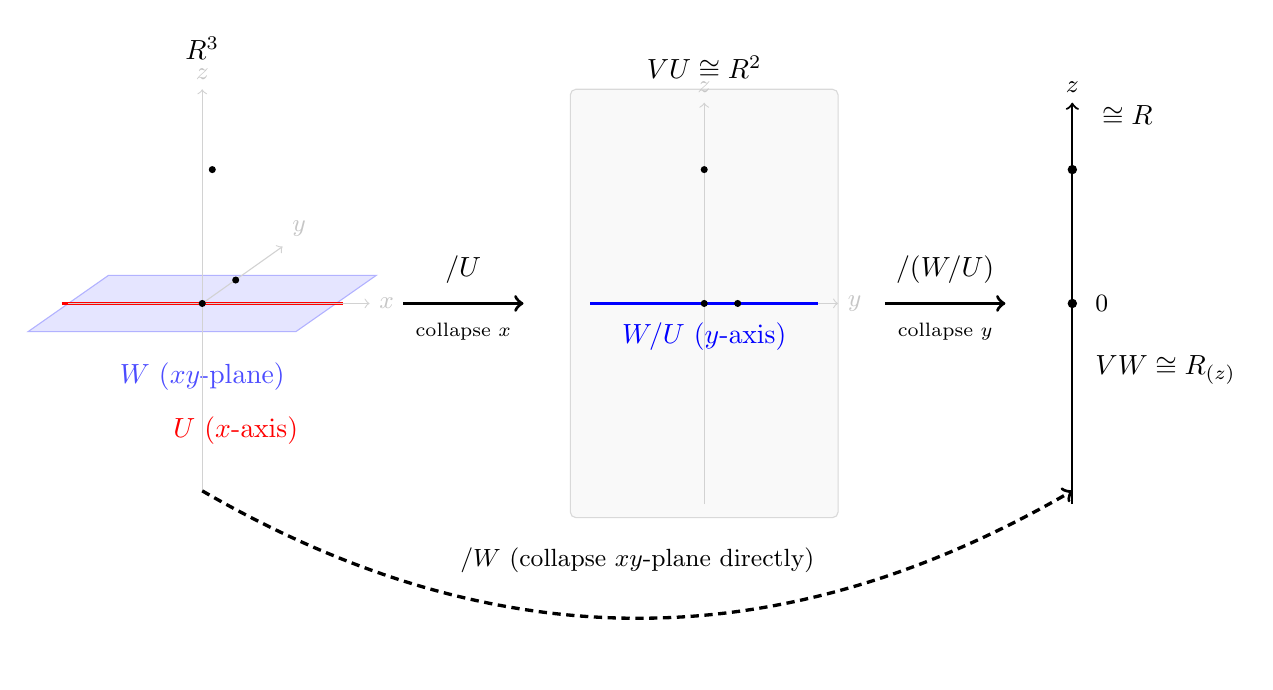
\begin{tikzpicture}[scale=0.85]
        % === Panel 1: R^3 (oblique projection) ===
        % Projection: x->(1,0), y->(0.5,0.35), z->(0,1)
        \node[above] at (0,3.5) {$\bb{R}^3$};

        % W (xy-plane) as tilted parallelogram
        % Corners: (±2, 0, 0) ± (0, 1.2, 0), with y->(0.5, 0.35)
        % so y offset = (0.6, 0.42)
        % (-2-0.6, -0.42), (2-0.6, -0.42), (2+0.6, 0.42), (-2+0.6, 0.42)
        \fill[blue!10] (-2.6,-0.42) -- (1.4,-0.42) -- (2.6,0.42) -- (-1.4,0.42) -- cycle;
        \draw[blue!30] (-2.6,-0.42) -- (1.4,-0.42) -- (2.6,0.42) -- (-1.4,0.42) -- cycle;
        \node[blue!70] at (0,-1.1) {$W$ ($xy$-plane)};

        % U (x-axis)
        \draw[red, thick] (-2.1,0) -- (2.1,0);
        \node[red] at (0.5,-1.9) {$U$ ($x$-axis)};

        % Axes
        \draw[->, gray!35] (-2,0) -- (2.5,0) node[right, gray!45] {\small $x$};
        \draw[->, gray!35] (0,-2.8) -- (0,3.2) node[above, gray!45] {\small $z$};
        \draw[->, gray!35] (0,0) -- (1.2,0.85) node[above right, gray!45] {\small $y$};

        % Sample points
        \fill (0.5,0.35) circle (1.5pt);
        \fill (0,0) circle (1.5pt);
        \fill (0.15,2.0) circle (1.5pt);

        % === Arrow 1 ===
        \draw[->, very thick] (3.0,0) -- (4.8,0);
        \node[above] at (3.9,0.15) {$/U$};
        \node[below, font=\scriptsize] at (3.9,-0.15) {collapse $x$};

        % === Panel 2: V/U = R^2 ===
        \draw[gray!30, fill=gray!5, rounded corners=2pt] (5.5,-3.2) rectangle (9.5,3.2);
        \node[above] at (7.5,3.2) {$\QuotientSpace{V}{U} \cong \bb{R}^2$};

        % Axes
        \draw[->, gray!35] (5.8,0) -- (9.5,0) node[right, gray!45] {\small $y$};
        \draw[->, gray!35] (7.5,-3) -- (7.5,3) node[above, gray!45] {\small $z$};

        % W/U (y-axis)
        \draw[blue, thick] (5.8,0) -- (9.2,0);
        \node[blue] at (7.5,-0.5) {$W/U$ ($y$-axis)};

        % Sample points
        \fill (8.0,0) circle (1.5pt);
        \fill (7.5,0) circle (1.5pt);
        \fill (7.5,2.0) circle (1.5pt);

        % === Arrow 2 ===
        \draw[->, very thick] (10.2,0) -- (12.0,0);
        \node[above] at (11.1,0.15) {$/(W/U)$};
        \node[below, font=\scriptsize] at (11.1,-0.15) {collapse $y$};

        % === Panel 3: R_(z) ===
        \draw[->, thick] (13,-3) -- (13,3) node[above] {\small $z$};
        \fill (13,2.0) circle (2pt);
        \fill (13,0) circle (2pt);
        \node[right] at (13.2,0) {\small $\EquivClass{0}$};
        \node[right] at (13.3,2.8) {$\cong \bb{R}$};
        \node[right] at (13.2,-1) {$\QuotientSpace{V}{W} \cong \bb{R}_{(z)}$};

        % === Direct path (bottom): smooth curved arc from R^3 to R_(z) ===
        \draw[->, very thick, densely dashed]
            (0,-2.8) to[out=-30, in=-150] (13,-2.8);
        \node[below, font=\small] at (6.5,-3.5)
            {$/W$ (collapse $xy$-plane directly)};
    \end{tikzpicture}
    \end{center}
\end{example}

\begin{remark}[Intuition for Third Isomorphism Theorem]
    The third isomorphism theorem says that ``quotients of quotients'' simplify.
    Intuitively: if we first collapse $U$ to a point, then collapse the image of $W$,
    we get the same result as collapsing $W$ directly.

    In finite dimensions with $\Dim[K]{V} = n$, $\Dim[K]{W} = m$, $\Dim[K]{U} = k$ (where $k \leq m \leq n$):
    \begin{align*}
        \Dim[K]{\QuotientSpace{V}{U}} &= n - k \\
        \Dim[K]{\QuotientSpace{W}{U}} &= m - k \\
        \Dim[K]{\QuotientSpace{\QuotientSpace p{V}{U}}{\QuotientSpace p{W}{U}}} &= (n-k) - (m-k) = n - m = \Dim[K]{\QuotientSpace{V}{W}}
    \end{align*}
\end{remark}

\subsection{Fourth Isomorphism Theorem (Lattice Correspondence)}

\begin{remark}[Motivation]
    The previous theorems constructed specific isomorphisms between quotient spaces. The
    fourth theorem is different in character: it is a \textbf{structural correspondence}
    between the subspaces of a quotient $\QuotientSpace{V}{W}$ and the subspaces of $V$
    that contain $W$. This is the linear-algebraic analogue of the correspondence theorem
    for groups and rings.

    The practical import is that we can study the internal structure of a quotient space
    without ever leaving $V$: every subspace $X \Subspace[K] \QuotientSpace{V}{W}$
    ``lifts'' to a unique subspace $U \Subspace[K] V$ with $W \subseteq U$, and the
    operations of sum and intersection are preserved. This makes the fourth isomorphism
    theorem an indispensable tool for inductive arguments and for analyzing chains of
    subspaces (flags) in quotient spaces.
\end{remark}

\begin{theorem}[Fourth Isomorphism Theorem]\label{thm:fourth-iso}
    Let $W \Subspace[K] V$. There is a bijective correspondence between:
    \begin{itemize}
        \item Subspaces of $\QuotientSpace{V}{W}$
        \item Subspaces of $V$ containing $W$
    \end{itemize}

    Equivalently, the subspace lattice of $\QuotientSpace{V}{W}$ is isomorphic
    to the sublattice of $\SubspaceLattice{V}$ bounded below by $W$:
    \[
        \SubspaceLattice{\QuotientSpace{V}{W}} \;\cong\; \Set{U \in \SubspaceLattice{V} \mid W \subseteq U}
    \]

    The correspondence is given by:
    \begin{align*}
        \Phi: \Set{U \in \SubspaceLattice{V} \mid W \subseteq U} &\to \SubspaceLattice{\QuotientSpace{V}{W}} \\
        U &\mapsto \QuotientSpace{U}{W} = \Set{\Coset{u}{W} \mid u \in U}
    \end{align*}
    with inverse:
    \begin{align*}
        \Psi: \SubspaceLattice{\QuotientSpace{V}{W}} &\to \Set{U \in \SubspaceLattice{V} \mid W \subseteq U} \\
        X &\mapsto \InverseImage{\pi}{X} = \Set{v \in V \mid \Coset{v}{W} \in X}
    \end{align*}

    Moreover, $\Phi$ is a lattice isomorphism --- it preserves:
    \begin{enumerate}
        \item Inclusion: $U_1 \subseteq U_2 \Leftrightarrow \Phi(U_1) \subseteq \Phi(U_2)$
        \item Join: $\Phi(U_1 + U_2) = \Phi(U_1) + \Phi(U_2)$
        \item Meet: $\Phi(U_1 \Intersect U_2) = \Phi(U_1) \Intersect \Phi(U_2)$
        \item Dimension: $\Dim[K]{\Phi(U)} = \Dim[K]{\QuotientSpace{U}{W}}$
    \end{enumerate}
\end{theorem}

\begin{proof}
    We prove (a) well-definedness of both maps, (b) that they are mutual inverses,
    and (c) that both are lattice homomorphisms.

    \textbf{(a) Well-definedness.}

    \textbf{$\Phi$ is well-defined:}
    If $U \Subspace[K] V$ with $W \subseteq U$, then $\QuotientSpace{U}{W} = \Set{\Coset{u}{W} \mid u \in U}$
    is a subspace of $\QuotientSpace{V}{W}$.
    Indeed: $\Coset{0}{W} \in \QuotientSpace{U}{W}$, and
    $a\Coset{u_1}{W} + b\Coset{u_2}{W} = \Coset{au_1 + bu_2}{W} \in \QuotientSpace{U}{W}$
    for $u_1, u_2 \in U$ and $a, b \in K$.

    \textbf{$\Psi$ is well-defined:}
    For any subspace $X \Subspace[K] \QuotientSpace{V}{W}$, the preimage
    $\InverseImage{\pi}{X}$ is a subspace of $V$ (Proposition~\ref{prop:image-preimage-subspace}).

    Since $\Coset{0}{W} \in X$ (because $X$ is a subspace), we have
    $W = \InverseImage{\pi}{\Set{\Coset{0}{W}}} \subseteq \InverseImage{\pi}{X}$.
    Thus $W \subseteq \InverseImage{\pi}{X}$.

    \textbf{(b) $\Phi$ and $\Psi$ are mutual inverses.}

    \textbf{$\Psi \circ \Phi = \Identity{\Set{U \in \SubspaceLattice{V} \mid W \subseteq U}}$:}
    For $U \Subspace[K] V$ with $W \subseteq U$:
    \begin{align*}
        \Psi(\Phi(U)) &= \Psi(\QuotientSpace{U}{W}) \\
                      &= \Set{v \in V \mid \Coset{v}{W} \in \QuotientSpace{U}{W}} \\
                      &= \Set{v \in V \mid \Exists :{u \in U}{\Coset{v}{W} = \Coset{u}{W}}} \\
                      &= \Set{v \in V \mid \Exists :{u \in U}{v - u \in W}} \\
                      &= \Set{v \in V \mid v \in U + W} \\
                      &= U + W = U
    \end{align*}
    The last equality holds because $W \subseteq U$ implies $U + W = U$.

    \textbf{$\Phi \circ \Psi = \Identity{\SubspaceLattice{\QuotientSpace{V}{W}}}$:}
    For $X \Subspace[K] \QuotientSpace{V}{W}$:
    \begin{align*}
        \Phi(\Psi(X)) &= \Phi(\InverseImage{\pi}{X}) \\
                      &= \Set{\Coset{v}{W} \mid v \in \InverseImage{\pi}{X}} \\
                      &= \Set{\Coset{v}{W} \mid \Coset{v}{W} \in X} \\
                      &= X
    \end{align*}

    \textbf{(c) Both $\Phi$ and $\Psi$ are lattice homomorphisms.}

    We prove that each map preserves inclusion, join (sum), and meet (intersection).

    \textbf{$\Phi$ preserves inclusion:}
    If $U_1 \subseteq U_2$, then every coset $\Coset{u}{W}$ with $u \in U_1$ also has
    $u \in U_2$, so $\Phi(U_1) \subseteq \Phi(U_2)$. Conversely, if
    $\Phi(U_1) \subseteq \Phi(U_2)$, apply $\Psi$ (which is order-preserving as a preimage)
    to get $U_1 = \Psi(\Phi(U_1)) \subseteq \Psi(\Phi(U_2)) = U_2$.

    \textbf{$\Phi$ preserves joins:}
    \begin{align*}
        \Coset{v}{W} \in \Phi(U_1 + U_2)
            &\Leftrightarrow v \in U_1 + U_2 \\
            &\Leftrightarrow v = u_1 + u_2 \text{ for some } u_1 \in U_1,\; u_2 \in U_2 \\
            &\Leftrightarrow \Coset{v}{W} = \Coset{u_1}{W} + \Coset{u_2}{W}
                \in \Phi(U_1) + \Phi(U_2)
    \end{align*}

    \textbf{$\Phi$ preserves meets:}
    ($\subseteq$): If $v \in U_1 \Intersect U_2$, then $\Coset{v}{W} \in \Phi(U_1)$ and
    $\Coset{v}{W} \in \Phi(U_2)$, so $\Coset{v}{W} \in \Phi(U_1) \Intersect \Phi(U_2)$.

    ($\supseteq$): If $\Coset{v}{W} \in \Phi(U_1) \Intersect \Phi(U_2)$, then
    $v \in \Psi(\Phi(U_1)) \Intersect \Psi(\Phi(U_2)) = U_1 \Intersect U_2$, so
    $\Coset{v}{W} \in \Phi(U_1 \Intersect U_2)$.

    \textbf{$\Psi$ preserves inclusion:}
    If $X_1 \subseteq X_2$, then
    $\Psi(X_1) = \InverseImage{\pi}{X_1} \subseteq \InverseImage{\pi}{X_2} = \Psi(X_2)$,
    since preimages preserve inclusion. Conversely, if $\Psi(X_1) \subseteq \Psi(X_2)$,
    apply $\Phi$ to get $X_1 = \Phi(\Psi(X_1)) \subseteq \Phi(\Psi(X_2)) = X_2$.

    \textbf{$\Psi$ preserves joins:}
    We show $\Psi(X_1 + X_2) = \Psi(X_1) + \Psi(X_2)$.

    ($\supseteq$): If $v_1 \in \Psi(X_1)$ and $v_2 \in \Psi(X_2)$, then
    $\Coset{v_1}{W} \in X_1$ and $\Coset{v_2}{W} \in X_2$. So
    $\pi(v_1 + v_2) = \Coset{v_1}{W} + \Coset{v_2}{W} \in X_1 + X_2$,
    hence $v_1 + v_2 \in \Psi(X_1 + X_2)$.

    ($\subseteq$): If $v \in \Psi(X_1 + X_2)$, then $\Coset{v}{W} \in X_1 + X_2$,
    so $\Coset{v}{W} = \bar{x}_1 + \bar{x}_2$ for some $\bar{x}_1 \in X_1$,
    $\bar{x}_2 \in X_2$. Since $\pi$ is surjective, pick $v_1, v_2 \in V$ with
    $\pi(v_1) = \bar{x}_1$ and $\pi(v_2) = \bar{x}_2$. Then $v_1 \in \Psi(X_1)$,
    $v_2 \in \Psi(X_2)$, and $\pi(v - v_1 - v_2) = \Coset{0}{W}$, so
    $w \defeq v - v_1 - v_2 \in W \subseteq \Psi(X_1)$. Therefore
    $v = (v_1 + w) + v_2 \in \Psi(X_1) + \Psi(X_2)$.

    \textbf{$\Psi$ preserves meets:}
    We show $\Psi(X_1 \Intersect X_2) = \Psi(X_1) \Intersect \Psi(X_2)$.

    ($\subseteq$): If $v \in \Psi(X_1 \Intersect X_2)$, then
    $\Coset{v}{W} \in X_1 \Intersect X_2$, so $\Coset{v}{W} \in X_1$ and
    $\Coset{v}{W} \in X_2$. Thus $v \in \Psi(X_1) \Intersect \Psi(X_2)$.

    ($\supseteq$): If $v \in \Psi(X_1) \Intersect \Psi(X_2)$, then
    $\Coset{v}{W} \in X_1$ and $\Coset{v}{W} \in X_2$, so
    $\Coset{v}{W} \in X_1 \Intersect X_2$, hence $v \in \Psi(X_1 \Intersect X_2)$.

    \textbf{Dimension:}
    Follows from $\Phi(U) = \QuotientSpace{U}{W}$ by definition.
\end{proof}

\begin{example}[Fourth Isomorphism Theorem in $\bb{R}^3$]\label{ex:fourth-iso}
    Let $V = \bb{R}^3$ and $W = \Span[\bb{R}]{\Set{\CanonicalVector{0}}}$ (the $x$-axis).
    Then $\QuotientSpace{V}{W} \cong \bb{R}^2$ (parameterized by $(y,z)$).

    The subspaces of $V$ containing $W$ are:
    \begin{itemize}
        \item $W$ itself (the $x$-axis)
        \item Every plane through the origin containing the $x$-axis
              (e.g., the $xy$-plane, the $xz$-plane, $\Span[\bb{R}]{\Set{\CanonicalVector{0}, \CanonicalVector{1} + \CanonicalVector{2}}}$, \ldots)
        \item $\bb{R}^3$
    \end{itemize}

    The subspaces of $\QuotientSpace{V}{W} \cong \bb{R}^2$ are:
    \begin{itemize}
        \item $\Set{0}$
        \item Every line through the origin in $\bb{R}^2$
        \item $\bb{R}^2$
    \end{itemize}

    The correspondence $\Phi$ maps:
    $W \mapsto \Set{0}$, each plane containing $W$ to the line it becomes after
    collapsing the $x$-axis, and $\bb{R}^3 \mapsto \bb{R}^2$.
    For instance, the $xy$-plane maps to the $y$-axis, the $xz$-plane maps to the $z$-axis.

    \begin{center}
    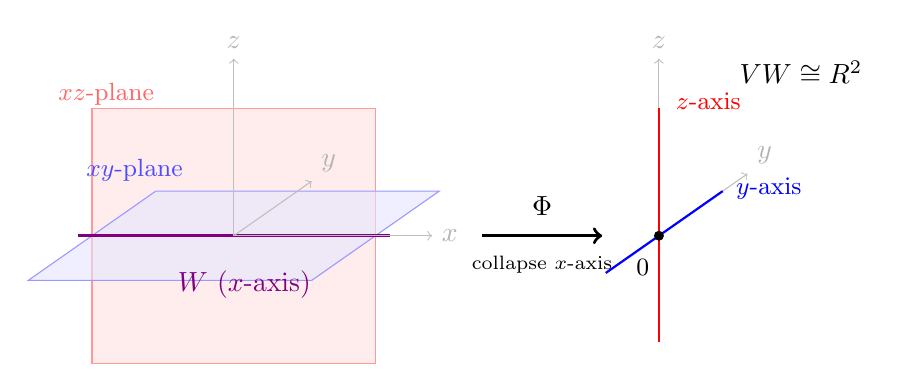
\begin{tikzpicture}[scale=0.9,
        x={(1cm,0cm)},
        y={(0.5cm,0.35cm)},
        z={(0cm,1cm)}]

        % --- Left: R^3 with W and planes containing W ---
        % Draw order: xz-plane (back), then xy-plane (front-tilted), then W on top

        % xz-plane (contains W) — behind, vertical
        \fill[red!10, opacity=0.7] (-2,0,-1.8) -- (2,0,-1.8) -- (2,0,1.8) -- (-2,0,1.8) -- cycle;
        \draw[red!40] (-2,0,-1.8) -- (2,0,-1.8) -- (2,0,1.8) -- (-2,0,1.8) -- cycle;
        \node[red!60] at (-1.8,0,2.0) {\small $xz$-plane};

        % xy-plane (contains W) — in front, tilted
        \fill[blue!10, opacity=0.6] (-2,-1.8,0) -- (2,-1.8,0) -- (2,1.8,0) -- (-2,1.8,0) -- cycle;
        \draw[blue!40] (-2,-1.8,0) -- (2,-1.8,0) -- (2,1.8,0) -- (-2,1.8,0) -- cycle;
        \node[blue!70] at (-2.3,1.8,0.3) {\small $xy$-plane};

        % W = x-axis, highlighted (on top of both planes)
        \draw[violet, very thick] (-2.2,0,0) -- (2.2,0,0);
        \node[violet] at (0,0.3,-0.8) {$W$ ($x$-axis)};

        % Axes
        \draw[->, gray!50] (0,0,0) -- (2.8,0,0) node[right, gray!60] {$x$};
        \draw[->, gray!50] (0,0,0) -- (0,2.2,0) node[above right, gray!60] {$y$};
        \draw[->, gray!50] (0,0,0) -- (0,0,2.5) node[above, gray!60] {$z$};

        % Arrow
        \draw[->, very thick] (3.5,0,0) -- (5.2,0,0);
        \node[above] at (4.35,0,0.15) {$\Phi$};
        \node[below, font=\scriptsize] at (4.35,0,-0.15) {collapse $x$-axis};

        % --- Right: V/W = R^2 with lines ---
        \draw[->, gray!50] (6,0,0) -- (6,2.5,0) node[above right, gray!60] {$y$};
        \draw[->, gray!50] (6,0,0) -- (6,0,2.5) node[above, gray!60] {$z$};

        % y-axis (image of xy-plane)
        \draw[blue, thick] (6,-1.5,0) -- (6,1.8,0);
        \node[blue, right] at (6,1.9,0) {\small $y$-axis};

        % z-axis (image of xz-plane)
        \draw[red, thick] (6,0,-1.5) -- (6,0,1.8);
        \node[red, right] at (6.1,0,1.9) {\small $z$-axis};

        % Origin
        \fill (6,0,0) circle (2pt);
        \node[below left] at (6,0,-0.2) {\small $\Set{0}$};

        \node[right] at (7,0,2.3) {$\QuotientSpace{V}{W} \cong \bb{R}^2$};
    \end{tikzpicture}
    \end{center}

    \begin{center}
    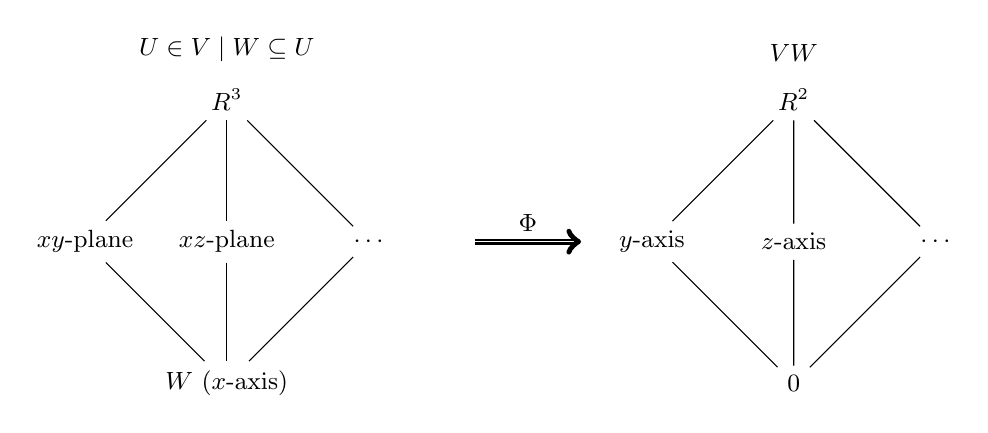
\begin{tikzpicture}[scale=0.9, every node/.style={font=\small}]
        % Left lattice: Sub(V) above W
        \node (V) at (0,4) {$\bb{R}^3$};
        \node (xy) at (-2,2) {$xy$-plane};
        \node (xz) at (0,2) {$xz$-plane};
        \node (xd) at (2,2) {$\cdots$};
        \node (W) at (0,0) {$W$ ($x$-axis)};

        \draw (V) -- (xy);
        \draw (V) -- (xz);
        \draw (V) -- (xd);
        \draw (xy) -- (W);
        \draw (xz) -- (W);
        \draw (xd) -- (W);

        \node[above] at (0,4.4) {$\Set{U \in \SubspaceLattice{V} \mid W \subseteq U}$};

        % Arrow
        \draw[->, thick, double] (3.5,2) -- (5,2) node[midway, above] {$\Phi$};

        % Right lattice: Sub(V/W)
        \node (R2) at (8,4) {$\bb{R}^2$};
        \node (ly) at (6,2) {$y$-axis};
        \node (lz) at (8,2) {$z$-axis};
        \node (ld) at (10,2) {$\cdots$};
        \node (0) at (8,0) {$\Set{0}$};

        \draw (R2) -- (ly);
        \draw (R2) -- (lz);
        \draw (R2) -- (ld);
        \draw (ly) -- (0);
        \draw (lz) -- (0);
        \draw (ld) -- (0);

        \node[above] at (8,4.4) {$\SubspaceLattice{\QuotientSpace{V}{W}}$};
    \end{tikzpicture}
    \end{center}
\end{example}

\begin{remark}[Lattice Interpretation]
    The fourth isomorphism theorem says that the subspace lattice $\SubspaceLattice{\QuotientSpace{V}{W}}$
    is isomorphic to the \textbf{principal filter} ${\uparrow}W = \Set{U \in \SubspaceLattice{V} \mid W \subseteq U}$
    in $\SubspaceLattice{V}$---that is, the portion of the lattice of $V$ that lies above $W$.

    Quotienting by $W$ ``cuts off'' everything below $W$ in the lattice and relabels what remains.
    The lattice operations are preserved:
    \begin{itemize}
        \item Join (supremum): $U_1 \vee U_2 = U_1 + U_2$
        \item Meet (infimum): $U_1 \wedge U_2 = U_1 \Intersect U_2$
    \end{itemize}

    This is particularly useful when analyzing quotient spaces by examining the subspace
    structure above $W$: every question about subspaces of $\QuotientSpace{V}{W}$ can be
    translated into a question about subspaces of $V$ containing $W$, and vice versa.
\end{remark}
